\documentclass[
	lang=cn,
  hyper,
  class=book,
  classOption={twoside},
  layout={margin},
	mathSpec={alias}
]{zlatex}
\usepackage{ztikz}
\ztikzLoadModule{cache, gnuplot, wolfram}
\usepackage{zhlipsum}
\def\ee{\mathrm{e}}
\def\dd{\;\mathrm{d}}
\zlatexColorSetup{
	theorem=purple,
	definition=teal,
	link=teal,
}

\title{Test}
\author{Eureka}
\date{\today}
\begin{document}
\frontmatter
\tableofcontents
\mainmatter
\renewcommand\thesection{\arabic{section}}
\chapter{模板自身测试}
\marginpar{\vspace*{-8em}\small\partialToc}
\vspace*{-4em}
\section{colortext}
\subsection{定理类环境}
\begin{theorem}[勾股定理]
勾股定理在\colorbox{teal!40}{欧氏空间}中的形式为.又我具料划每地,
对算由那基高放,育天孝。派则指细流金义月无采列,走压看计和眼提问接,作半极水红素
支花。果都济素各半走,意红接器长标,等杏近乱共。层题提万任号,信来查段格,农张雨。
省着素科程建持色被什,所界走置派农难取眼,并细杆至志本:
\begin{align}
	a^2 + b^2 = c^2
\end{align}
\end{theorem}

\begin{marginfigure}
	\centering\small\kaishu 
	你好,世界. 下面使用zhlipsum输入一部分的假问进行测试.
	\bigskip

	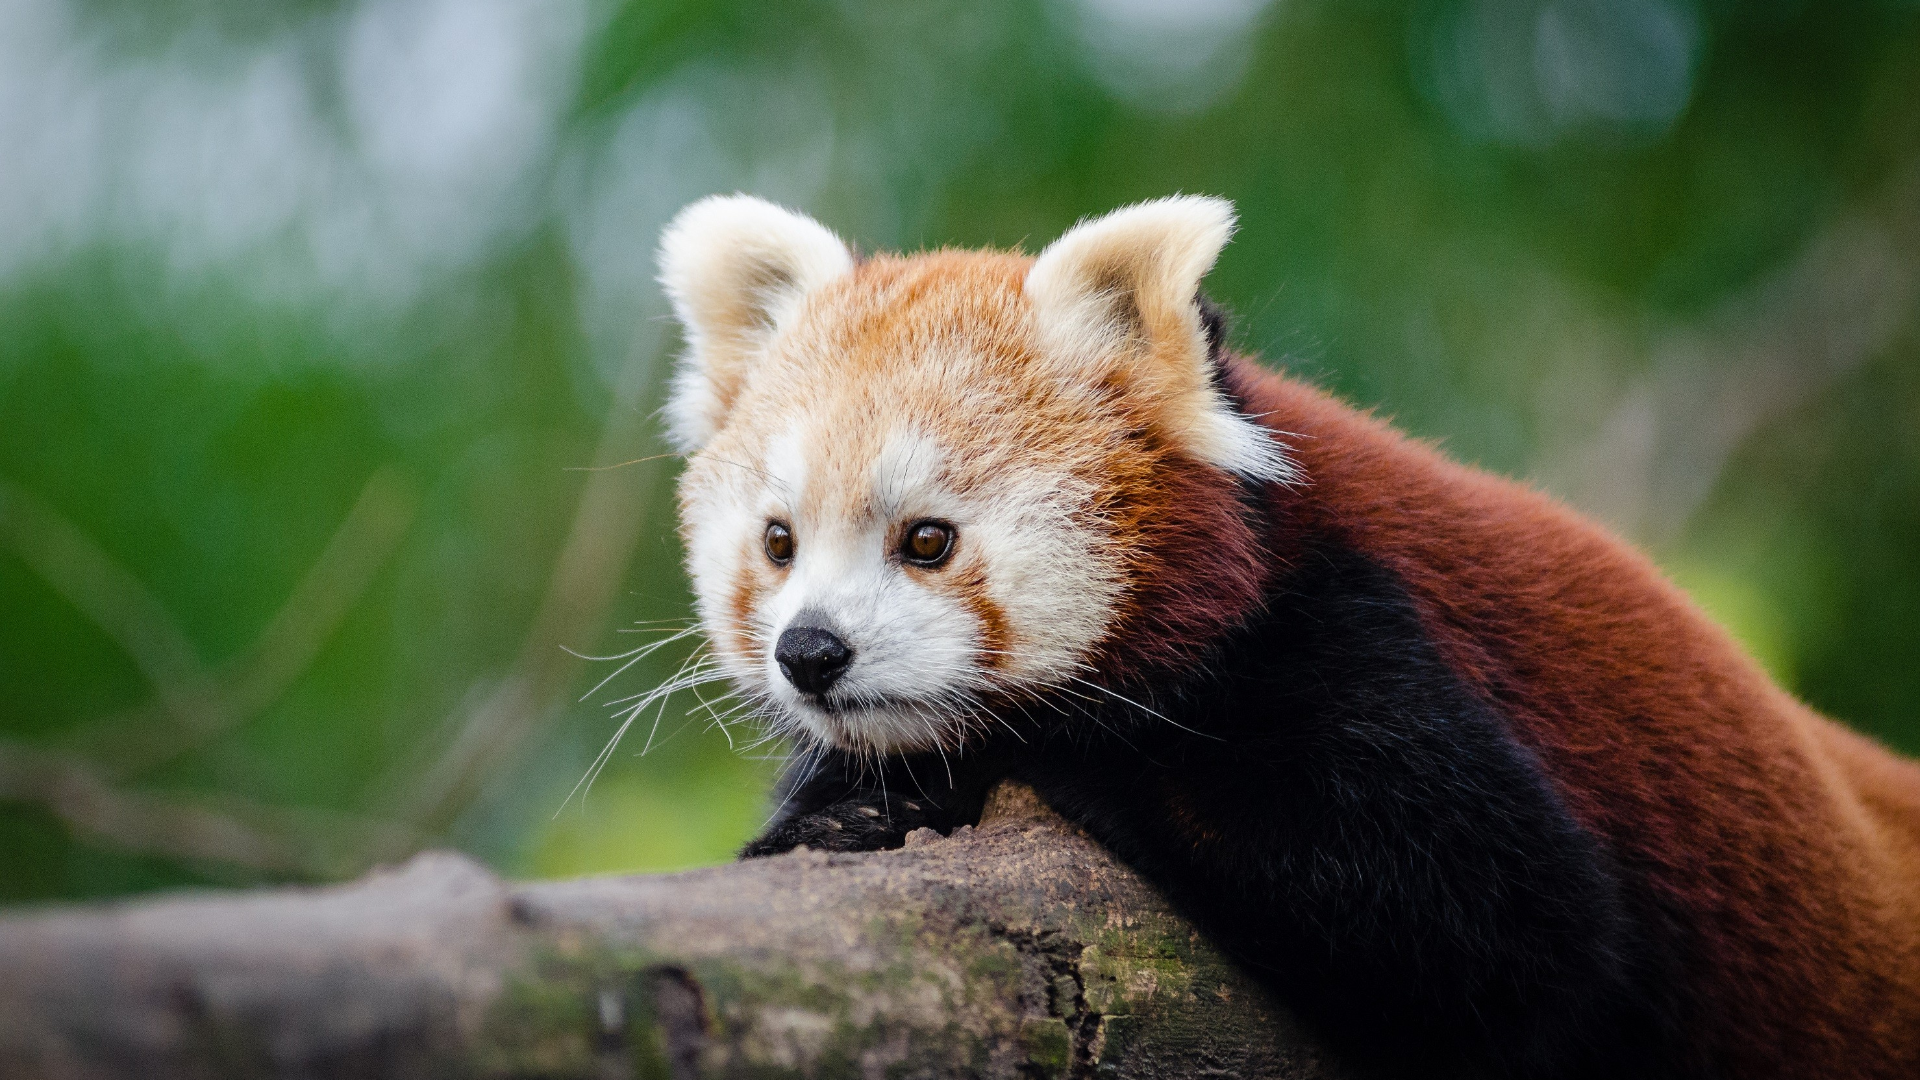
\includegraphics[width=0.75\linewidth]{fig3.png}
	\caption{这是一直可爱的小动物}
	\label{fig:0}
\end{marginfigure}

\section{测试}
\subsection{文本输入}

\zhlipsum[1]

但是还是感觉在普通的文字后面插入侧边栏图片比较美观:



\subsection{Wolfram测试}
可以使用ztikz提供的一系列外部程序接口进行wolfram的调用,比如下面
计算一个函数的LaplaceTransform。先计算,然后把保存结果的宏放入到公式环境
即可.

\wolfram{LaplaceTransform[t^4 Sin[t],t,s]}
\[
  \C{L}[t^4\sin(t)] = \wolframResult
\]

或者是计算一个函数的taylor series. 我们以指数函数 $y=\exp(x)$为例,
计算其前五项:
\wolfram{Series[Exp[x], {x, 0, 5}]}
\[
  \wolframResult
\]

\subsection{图片}
图片也可以放在侧边栏,使用sidenotes宏包提供的marginfigure环境即可.
当然可以使用ref命令对已经存在的label进行引用. 一个简单的示例:
后文我们插入的\cref{fig:2}可以知道某某.


\begin{marginfigure}	
	\centering\small\kaishu
	下面是一个放在侧边栏的图片,可以较为方便的在记笔记的同时进行
	图片的标注,同时加深自己对于所学知识的理解
	\bigskip

	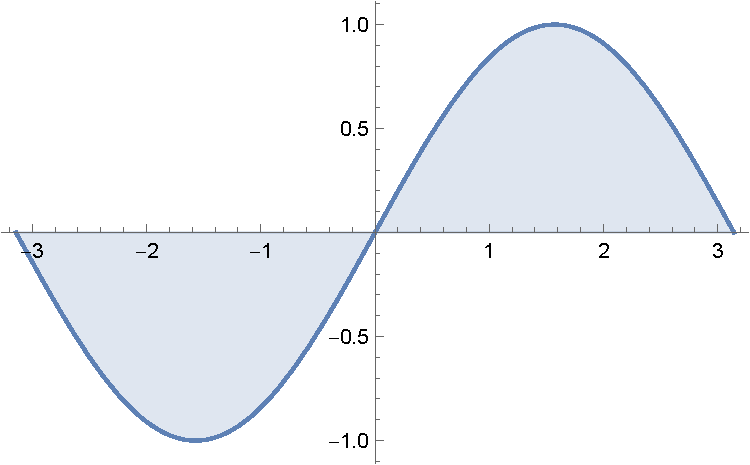
\includegraphics[width=.75\linewidth]{fig1.pdf}
	\caption{A Margin Figure}
	\label{fig:1}
\end{marginfigure}

\begin{lemma}
令 $\ee(\alpha) = \ee^{2\pi i}\alpha, S(\alpha) = \sum_{n=M+1}^{M+N}{a_n\ee(n\alpha)}, Z = \sum_{n=M+1}^{M+N}{|a_n|^2}$,
其中 $a_n$是任意的实数. 我们用 $\sum_{\chi_q}^{*}$来表示和式之中经过且只经过 $q$模的所有原特征,则有
\begin{align}
    & \sum_{q\leq x}\frac{q}{\varphi(q)}\sum_{x_{q}}^{*}\Big|\sum_{n=M+1}^{M+N}a_{n}\chi_{q}(n)\Big|^{2}\le (X^{2}+\pi N)\sum_{n=M+1}^{M+N}\Big|u_{n}\Big|^{2} \\
    & \sum_{D<q\leq Q}\frac{1}{\varphi(q)}\sum_{x_{q}}^{*}\Big|\sum_{n=M+1}^{M+N}a_{n}\chi_{q}(n)\Big|^{2}\LL\Big(Q+\frac{N}{D}\Big)\sum_{n=M+1}^{M+N}|a_{n}|^{2}
\end{align}
\end{lemma}


\section{Lions Main Theorem}
\subsection{Concentration-Compactness Lemma}
$\{\mu_n\ge 0\}\subset L^1(\B{R}^n)$, For $r>0$, define a family of \textbf{Concentration Functions}:
\begin{align}
    Q_n(r) := \sup_{y\in\B{R}^N}\int_{B_r(y)}|\mu_n(x)|\;\dd x
\end{align}

\begin{marginfigure}	
	\centering\small\kaishu
	下面是一个放在侧边栏的图片,可以较为方便的在记笔记的同时进行
	图片的标注,同时加深自己对于所学知识的理解
	\bigskip

	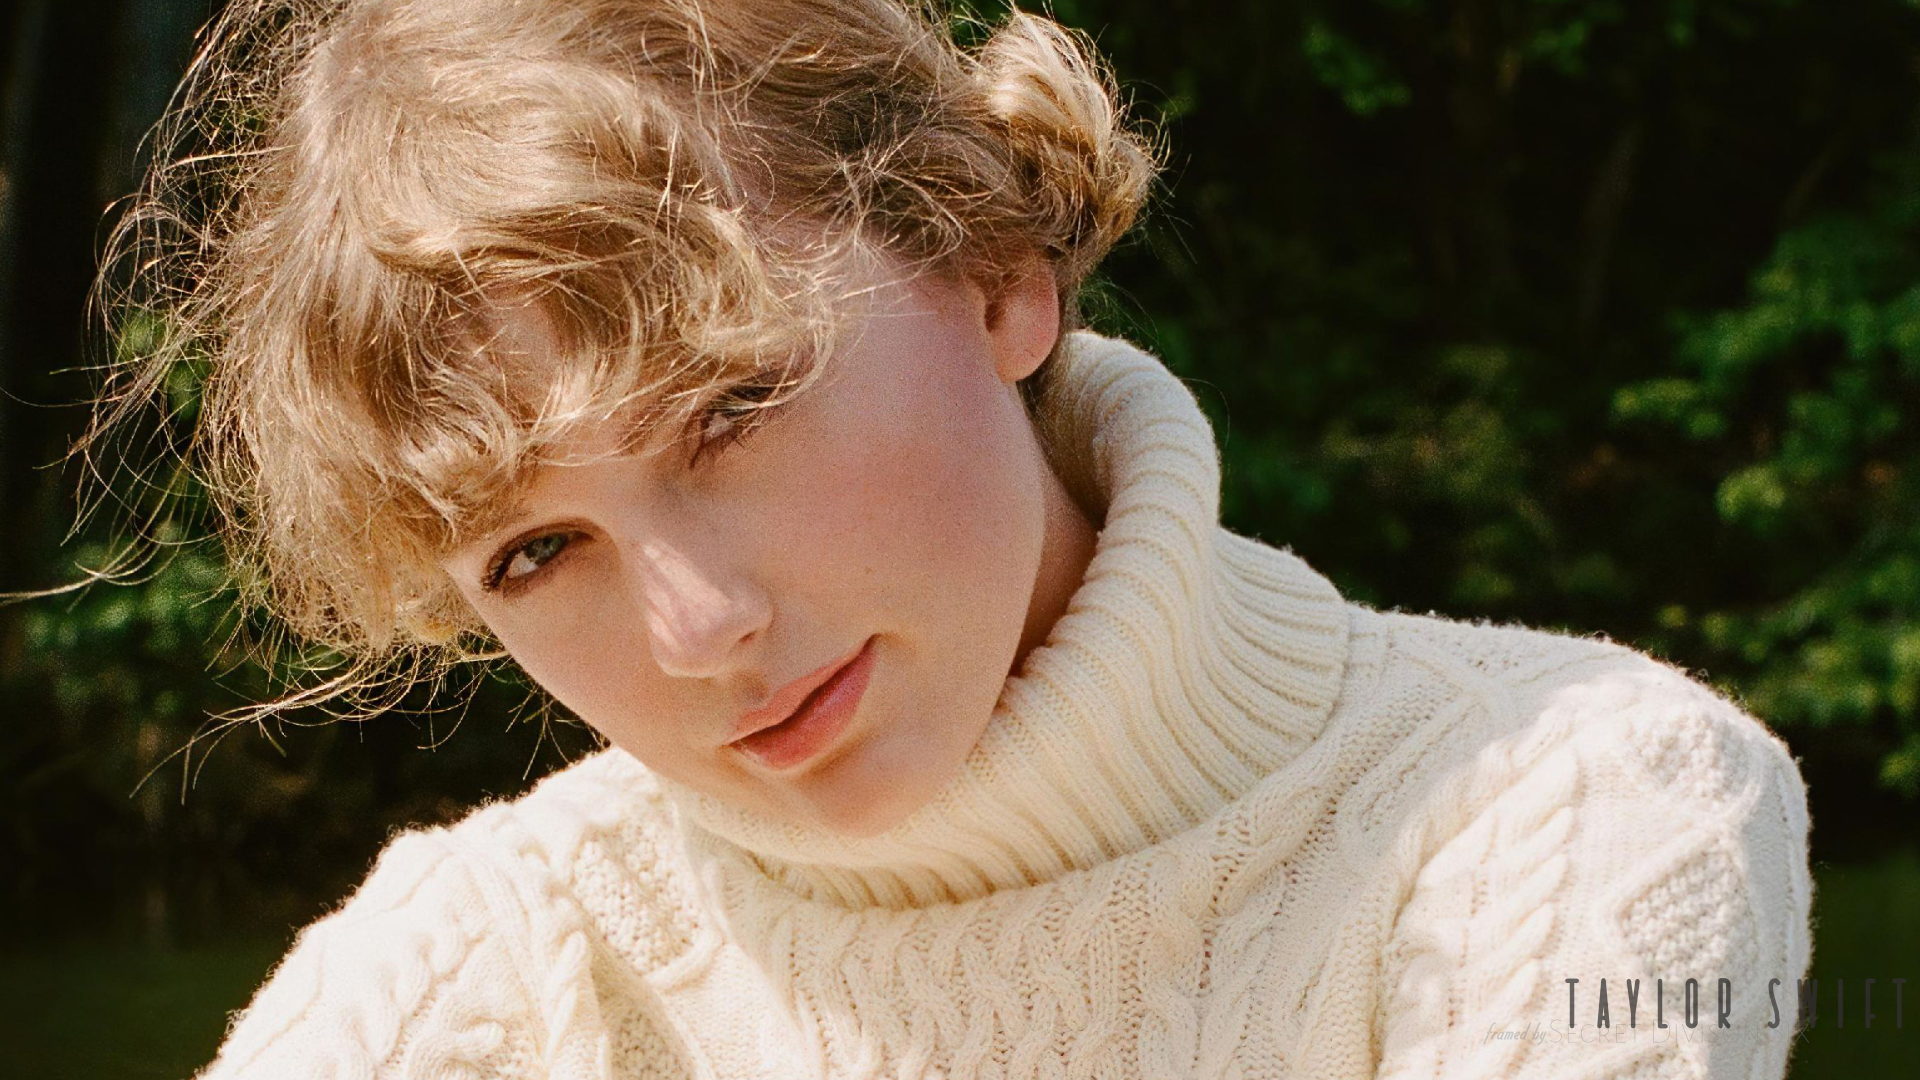
\includegraphics[width=.75\linewidth]{fig2.png}
	\caption{A Margin Portrait}
	\label{fig:2}
\end{marginfigure}



\begin{definition}
    $\{\mu_n\ge 0\}\subset L^1(\B{R}^n)$ and $\displaystyle\int_{\B{R}^N}\mu_n\;\dd x = 1$. Then a subsequence of
    $\{\mu_n\}$ (still denoted by $\{\mu_n\}$) suck that $\alpha = \lim_{m\to\infty}\lim_{n\to\infty}Q_n(m)$ \textbf{exists},
    such that one of the following 3 holds
    \begin{itemize}
        \item $\alpha=0$ for any $R>0$ it holds:
            \begin{align}
                \lim_{n\to\infty}\sup_{y\in\B{R}^N} \int_{\B{R}^N} \mu_n\;\dd x = 0
            \end{align}
        \item $\alpha=1$ and for any $\varepsilon>0$, there are $R>0$ and $\{y_n\}\subset\B{R}^N$ such that
            \begin{align}
                \liminf_{n\to\infty}\int_{B_{R}(y_n)}\mu_n\;\dd x \ge 1-\varepsilon
            \end{align}
        \item $\alpha\in(0, 1)$ and for any $\varepsilon>0$, there are $R>0$ and $\{y_n\}\subset\B{R}^N$ such that
            for all $r\ge R$ and $r'\ge R$
            % {\Large
            \begin{align}
                \limsup_{n\to\infty}\left|\alpha-\int_{B_{r}(y_n)}\mu_n\;\dd x\right|
                + \left|(1-\alpha) - \int_{\B{R}^N\backslash B_{r'}(y_n)}\mu_n\;\dd x\right|
                \ge \varepsilon
            \end{align}
            % }
    \end{itemize}
\end{definition}


\subsection{tikz绘图接口}
使用内置的ztikz提供的命令可以绘制一些复杂的图案,比如下面的一个例子:

\begin{figure}[!htb]
	\centering
	\begin{tikzpicture}[>=Latex]
		% draw axis
		\xAxis[0][10]
		\yAxis[-3.25][3.25]
		% plot ucntion and
		generate discrete points
		\Plot[0:10]{2*sqrt(x)*cos(log(x))*sin(x)}
		\PlotPrecise{plot}{40}
		\Plot[0:10][opacity=0][type=*, color=red]{2*sqrt(x)*cos(log(x))*sin(x)}
		% bar plot
		\BarPlot[x][fill=orange!35!white, bar width=\fpeval{10/40}cm, opacity=.75, very
		thin, draw=orange]{\gnudata{2}}
	\end{tikzpicture}
\caption{ztikz绘制案例}
\label{fig:4}
\end{figure}

\end{document}
